%!TeX root=../tese.tex
%("dica" para o editor de texto: este arquivo é parte de um documento maior)
% para saber mais: https://tex.stackexchange.com/q/78101

\chapter{Methodology}

The goal of this work is to explore the concept of extensibility on MSA and understand which components and concepts are key to develop an extensible software system. To reach it, it studies two software scenarios with different MSA solutions, comparing each solution for its design, development, and execution.

To do so, it was done in an iterative process with solution design, architecture implementation, metrics collection and evaluation, inspired by Design Science Research~\cite{DesignParad}.

\begin{figure}
    \centering
    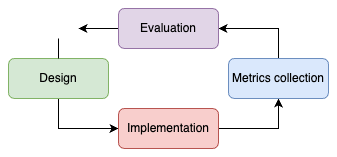
\includegraphics[width=.8\textwidth]{collector-consumer-Methodology.drawio}
    \caption{Methodology cycle.\label{fig:subfigures1}}
\end{figure}

During the solution design, the case study is selected and the architectures solutions are designed. Then, the architecture's microservices are implemented and integrated locally. Once the application is ready, it is executed on different tests according to the study case and metrics are collected in regards to development experience and runtime measurements. At the end of the iteration, the patterns are compared and the metrics collected are evaluated.

\begin{figure}
    \centering
    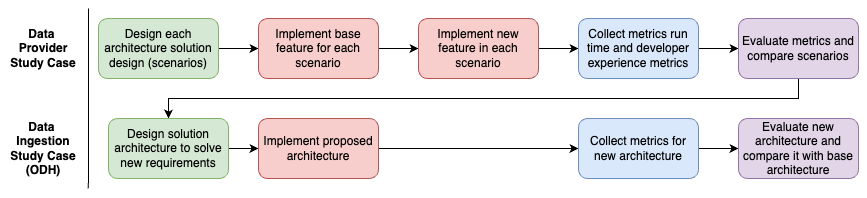
\includegraphics[width=1\textwidth]{collector-consumer-Methodology cycle.drawio}
    \caption{Iterations.\label{fig:subfigures2}}
\end{figure}

It was done in two iterations, each iteration was a case study where the use of microservices is required and extensibility is a non-functional requirement.

The first iteration was based on a common feature from multiple systems: to serve data to different clients. We named this case as “Data Provider”.

An initial solution is to protect the data source by exposing it as a service. The clients then access it via a REST API using a polling strategy. This study case compares it with two asynchronous approaches: a registration system that implements internally the broadcasting of the data exposed as REST API, and an event-based communication that delegates the broadcasting to a message broker.

The iteration started with the implementation of each scenario on a SpringBoot application according to the following GitHub's pull requests:

\begin{itemize}
    \item Polling gateway implementation: https://github.com/gfmota/charging-plug-gateway/pull/4
    \item Broadcaster gateway implementation: https://github.com/gfmota/charging-plug-gateway/pull/6
    \item Message-broker based implementation: https://github.com/gfmota/charging-plug-gateway/pull/1
\end{itemize}

Then, we wanted  to compare the technical effort necessary to extend the features in each scenario. So, we extended each scenario with a new microservice.

\begin{itemize}
    \item Polling provider new feature implementation: https://github.com/gfmota/charging-plug-gateway/pull/5
    \item Broadcaster provider new feature implementation: https://github.com/gfmota/charging-plug-gateway/pull/7
    \item Message-broker provider new feature implementation: https://github.com/gfmota/charging-plug-gateway/pull/8
\end{itemize}

During development, we collected developer experience metrics from a junior software engineer developing each provider. Such as, number of lines changed and knowledge necessary for each scenario. Due to the small sample, this may contain bias, and we encourage the experiment with a larger sample and a bigger context. 

After the implementation, each scenario was run locally in three clients usage battery, with 10, 100 and 1000 clients simultaneously for each one of the three data types provided. During runtime, we collected application’s health metrics from the data provider, such as CPU and memory usage, success and database access rate.

Then, we used the developer experience and runtime metrics to compare each scenario in regards to extensibility, scalability, data source usage, client autonomy and infrastructure cost.  

On the second iteration, the work studied the OpenDataHub's Data Ingestion use case. The Data Ingestion system is composed of several applications dedicated to collect and receive data from multiple external sources, transform them into a standardize structure and save on a common data storage.

We talked with the OpenDataHub's team to understand the current architecture, the requirements it met, and the desired requirements that are currently unfullfilled. 

Then, we designed a new architecture to accomodate both the old and the new requirements, and implemented it as followed on the GitHub's repository https://github.com/gfmota/data-ingestion-monorepo.

The implementation contains the integration of a Austrian Geosphere's dataset, provided by the OpenDataHub's team, as an example.

The implementation is used to simulate a dataset integration, active and passive integration, and to collect some analytical data about the new architecture. Then, we compared the current and the proposed architecture theoretically in regards to extensibility, work necessary to integrate a new dataset, and the system's functional requirements.
